% !TEX TS-program = xelatex
% !TEX encoding = UTF-8

\documentclass[a4paper, 11pt, twocolumn, draft]{article} % use larger type; default would be 10pt

\usepackage{default}

\defaultfontfeatures{Mapping=tex-text}
\setmainfont[Ligatures=TeX]{Linux Libertine}

% \usepackage[parfill]{parskip} % Activate to begin paragraphs with an empty line rather than an indent

\usepackage{graphicx} % support the \includegraphics command and options
\usepackage{bm}

\title{Principal Component Analysis and Competitive Learning of MNIST Data}
\author{Joe MacMahon, University of Sheffield}
\date{\today}

\begin{document}
\maketitle

\begin{abstract}

This report details my study and application Principal Component Analysis and
Competitive Learning to the MNIST data set of handwritten digits.

\end{abstract}

\section{Introduction}
% TODO reference MNIST

\section{PCA} A full introduction to PCA in any mathematical depth would be
outside the scope of this report, and can be found in any introductory machine
learning textbook.  However, we briefly state that PCA finds an ordering of
perpendicular axes (Principal Components) such that the projection of the data
onto the first principal component axis gives the largest spread of any
projection of the data, and each axis (a) is perpendicular to the rest and (b)
spreads the data wider than any subsequent axes.  Thus by composing a vector of
projections onto the ordered principal component axes, we obtain a vector whose
first component varies greatly with the data and each subsequent component
varies slightly less. For data of dimension $d$, this allows us to reduce its
dimensionality by considering the projection of the data onto the first $k$
principal component axes, for some $k < d$.  Through some mathematical
manipulation, it can be shown that the unit vectors of each principal component
axis are the eigenvectors of the covariance matrix of the data.

Using the Python library \texttt{numpy} to calculate a covariance matrix and
perform fast matrix multiplication, we perform PCA on the MNIST dataset and
take the first 5 principal components. Then we choose 3 of these 5 components
and plot them to a 3-D graph.\footnote{This answers question 1 of part 1.  For details of the algorithm and code snippets please see \autoref{sec:algorithms}.}  The results of this can be seen in
\autoref{fig:pca_graphs}.

\begin{figure}
  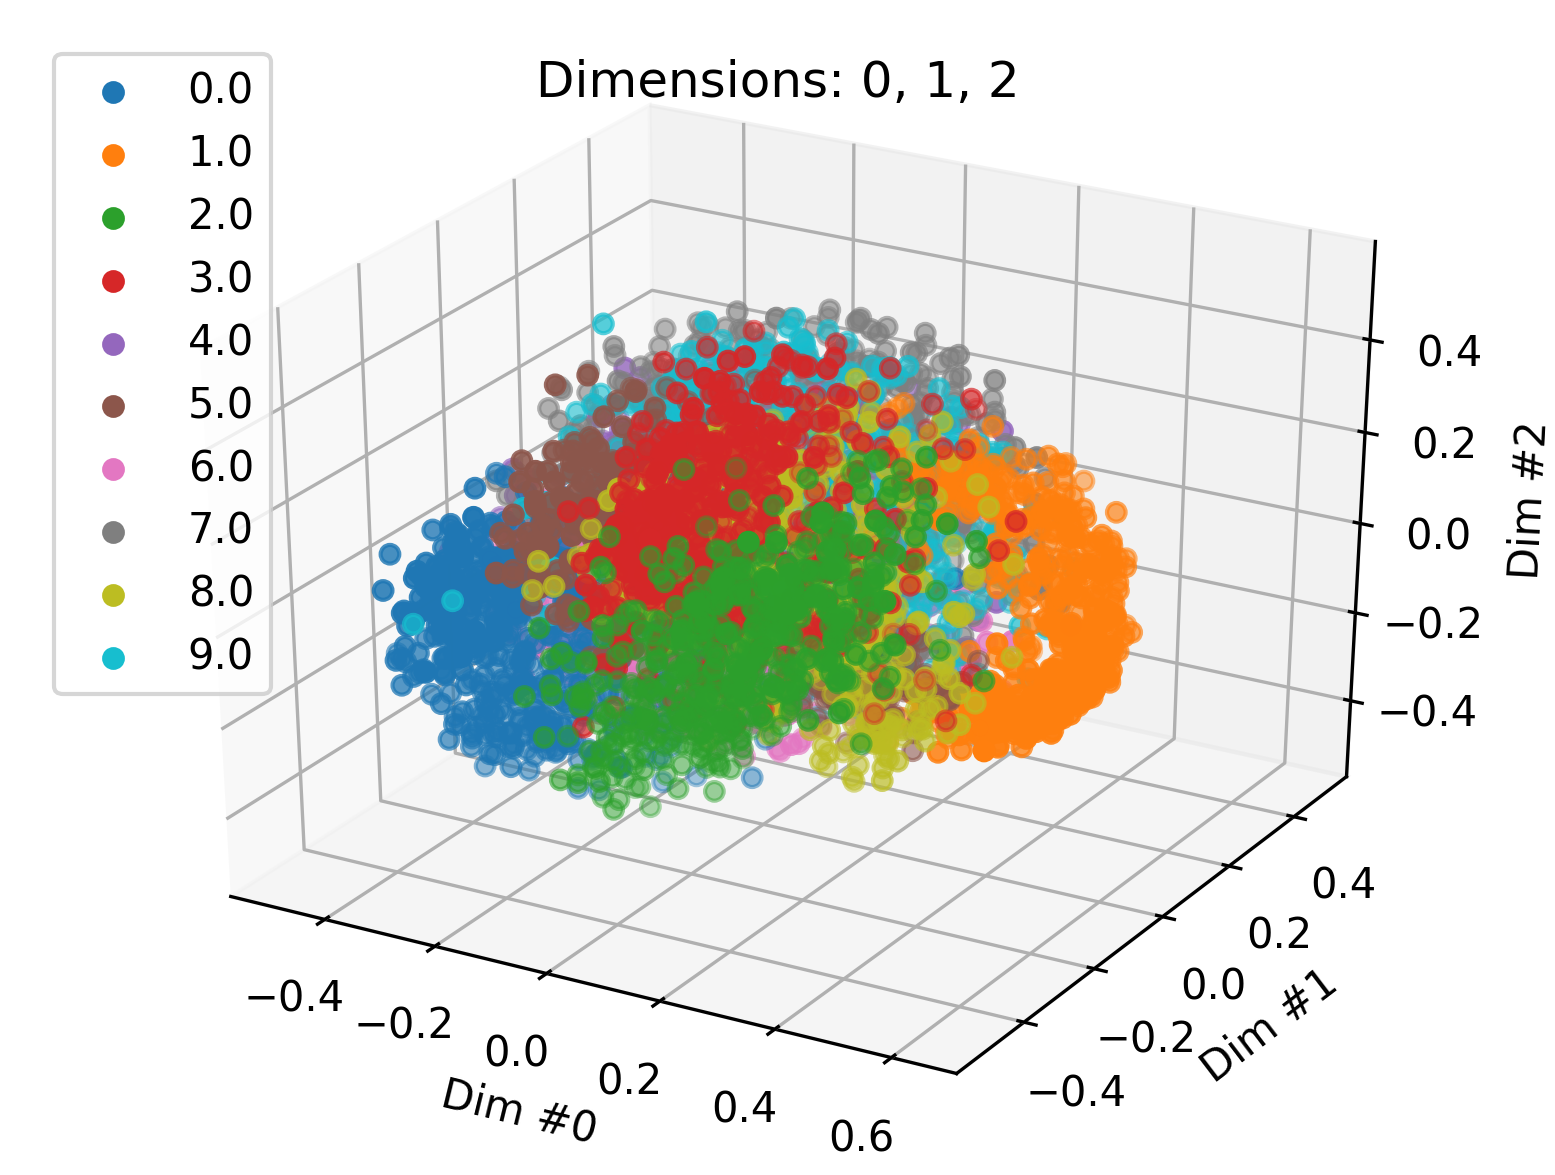
\includegraphics[width=0.23\textwidth]{pca/012.png}
  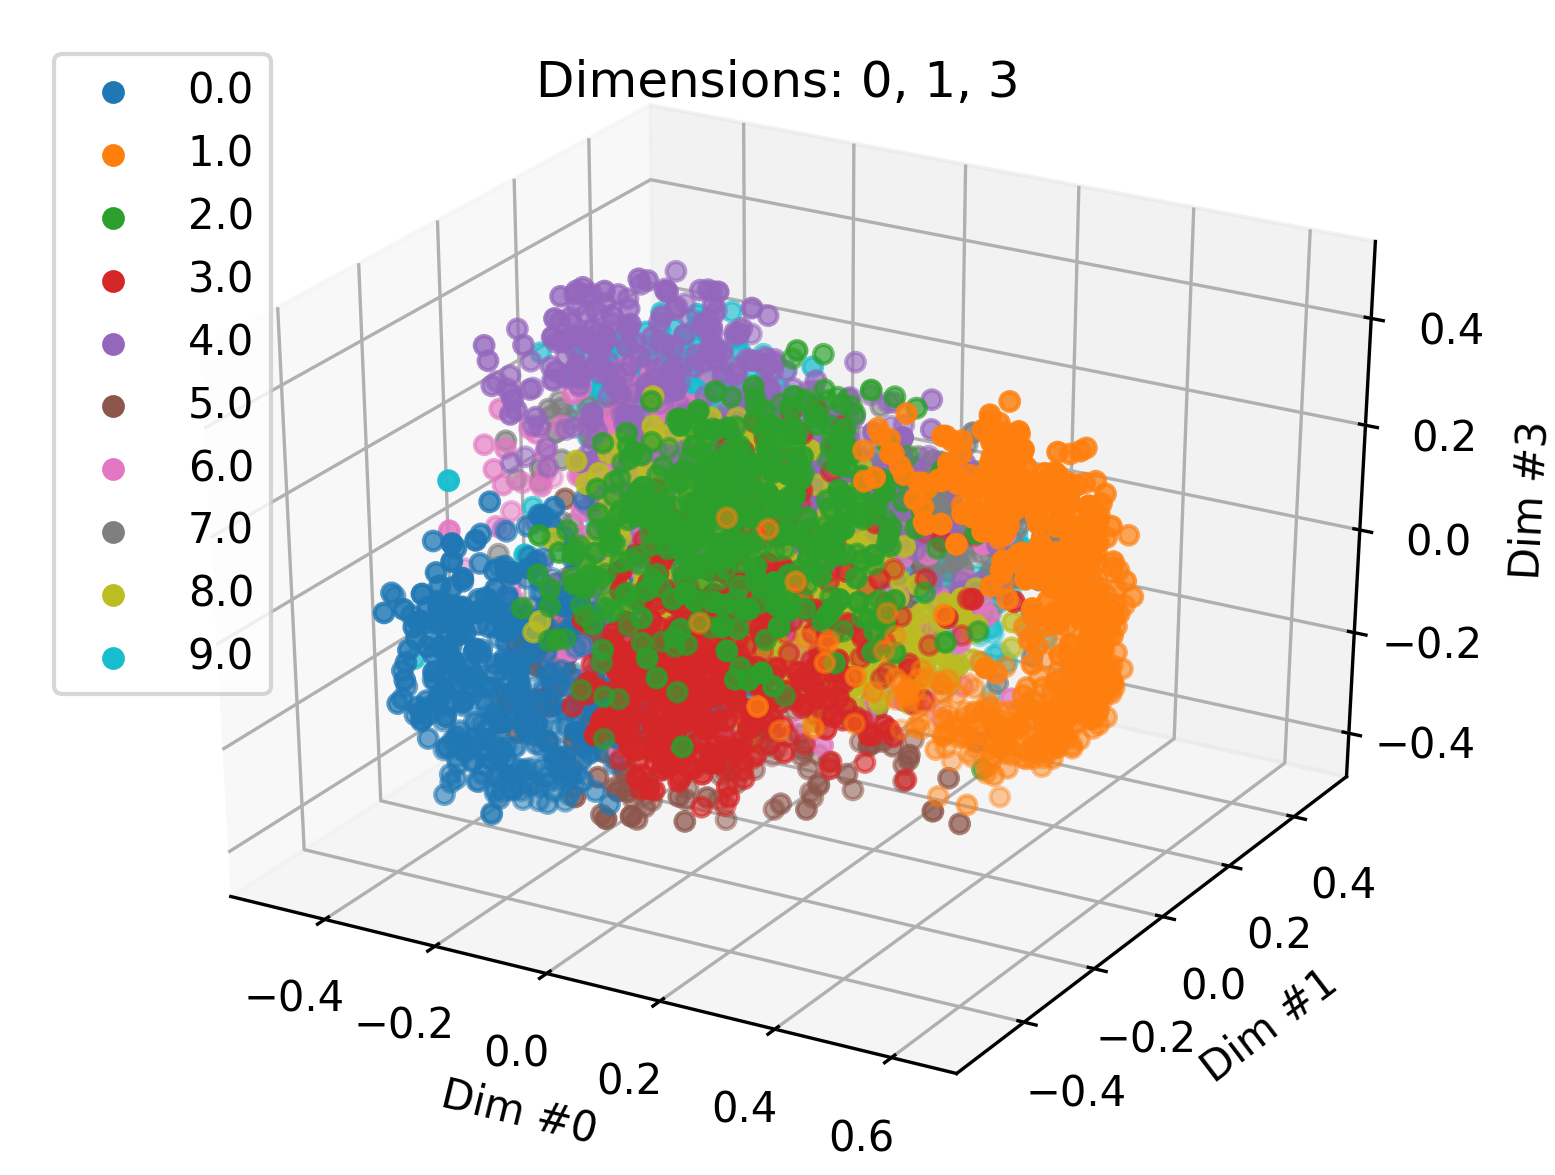
\includegraphics[width=0.23\textwidth]{pca/013.png}
  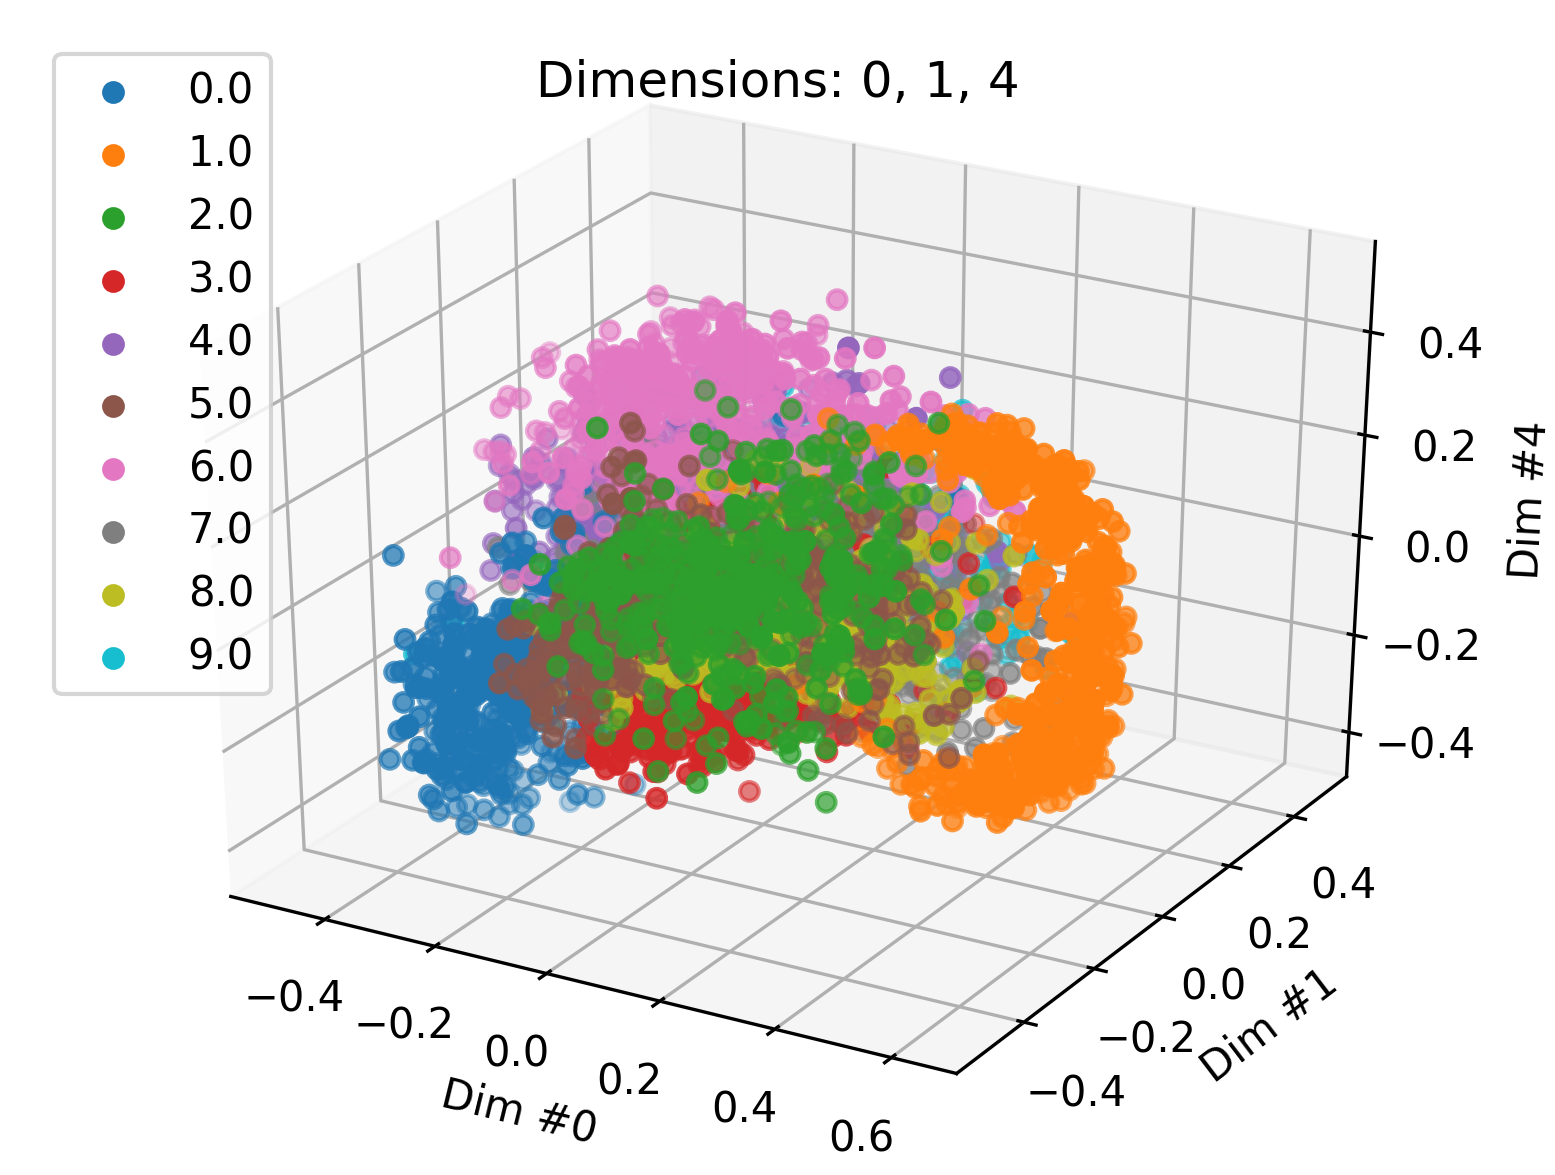
\includegraphics[width=0.23\textwidth]{pca/014.png}
  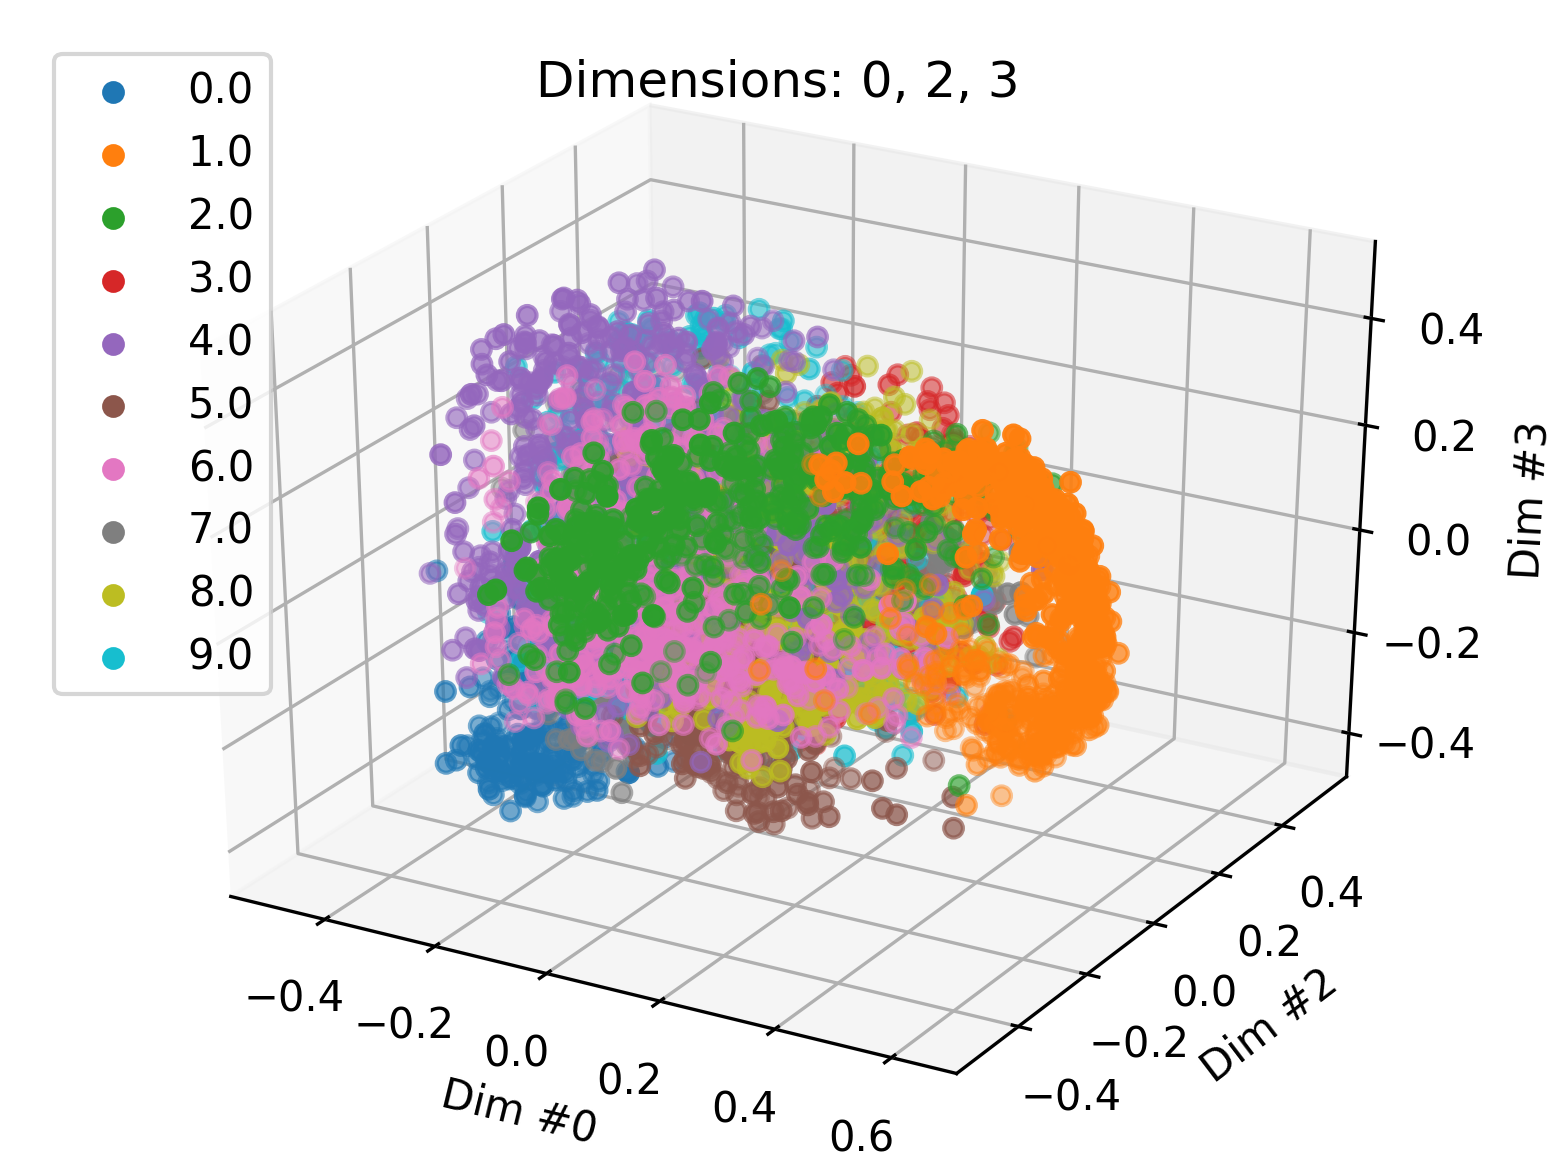
\includegraphics[width=0.23\textwidth]{pca/023.png}
  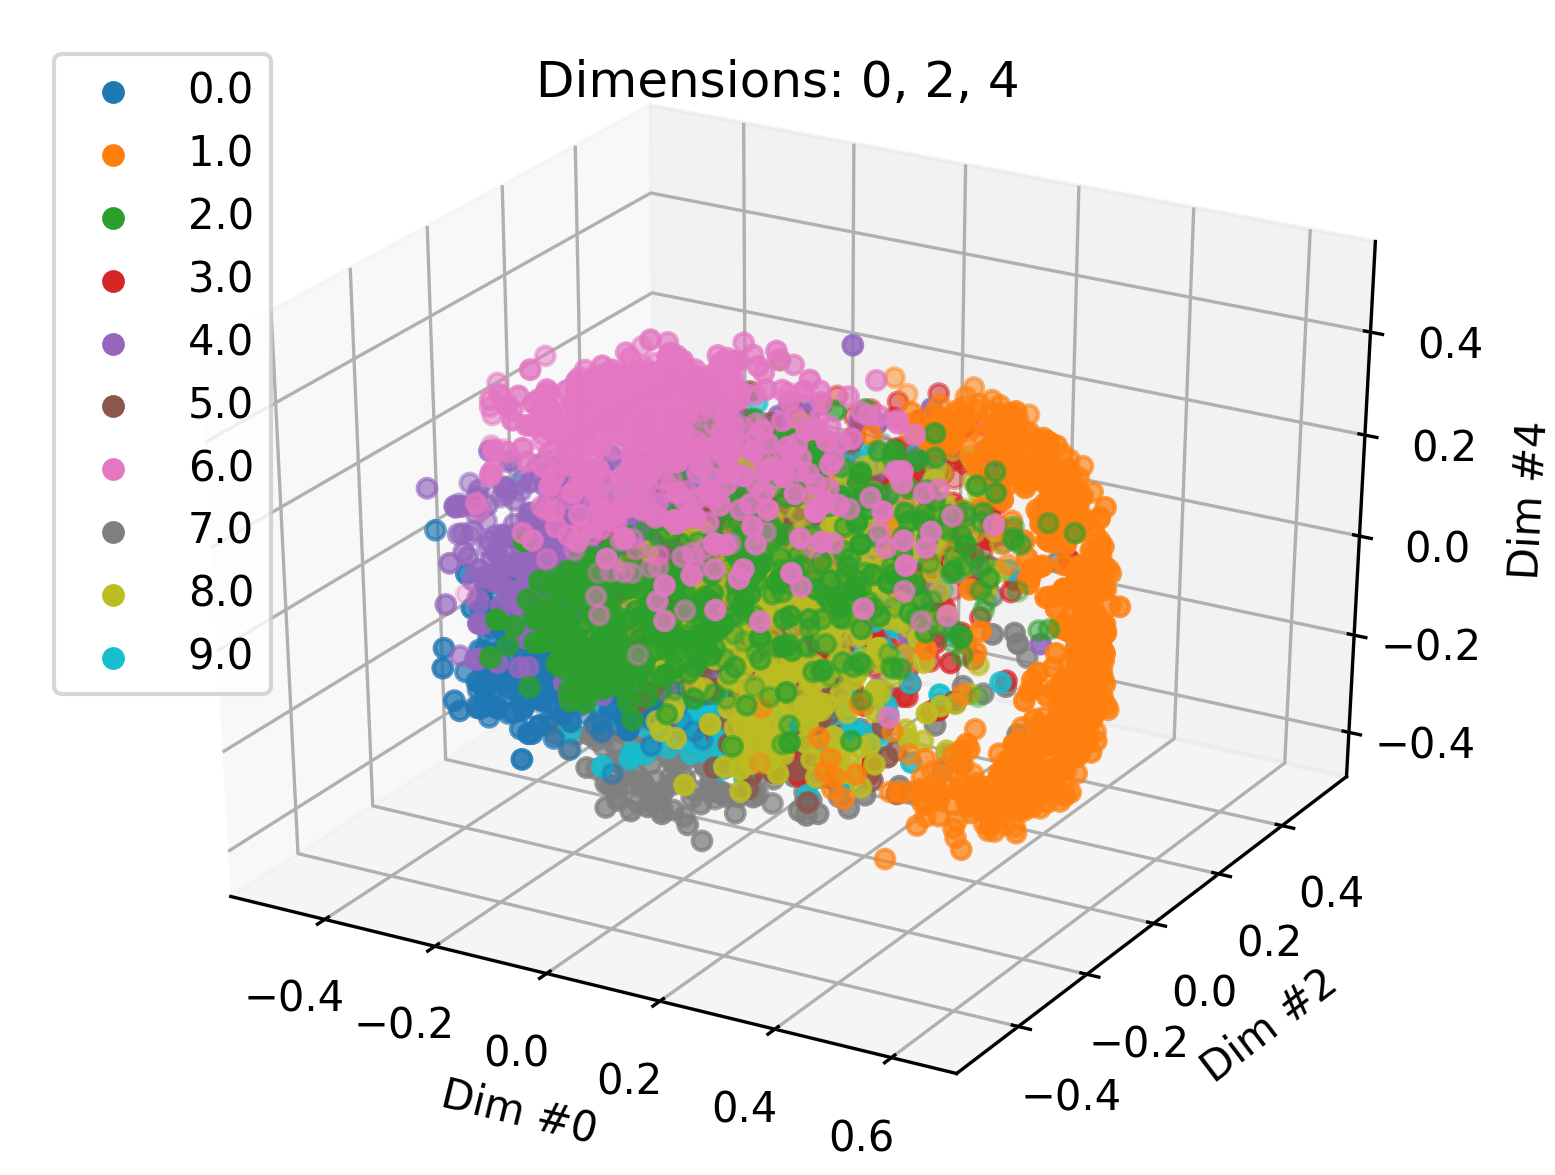
\includegraphics[width=0.23\textwidth]{pca/024.png}
  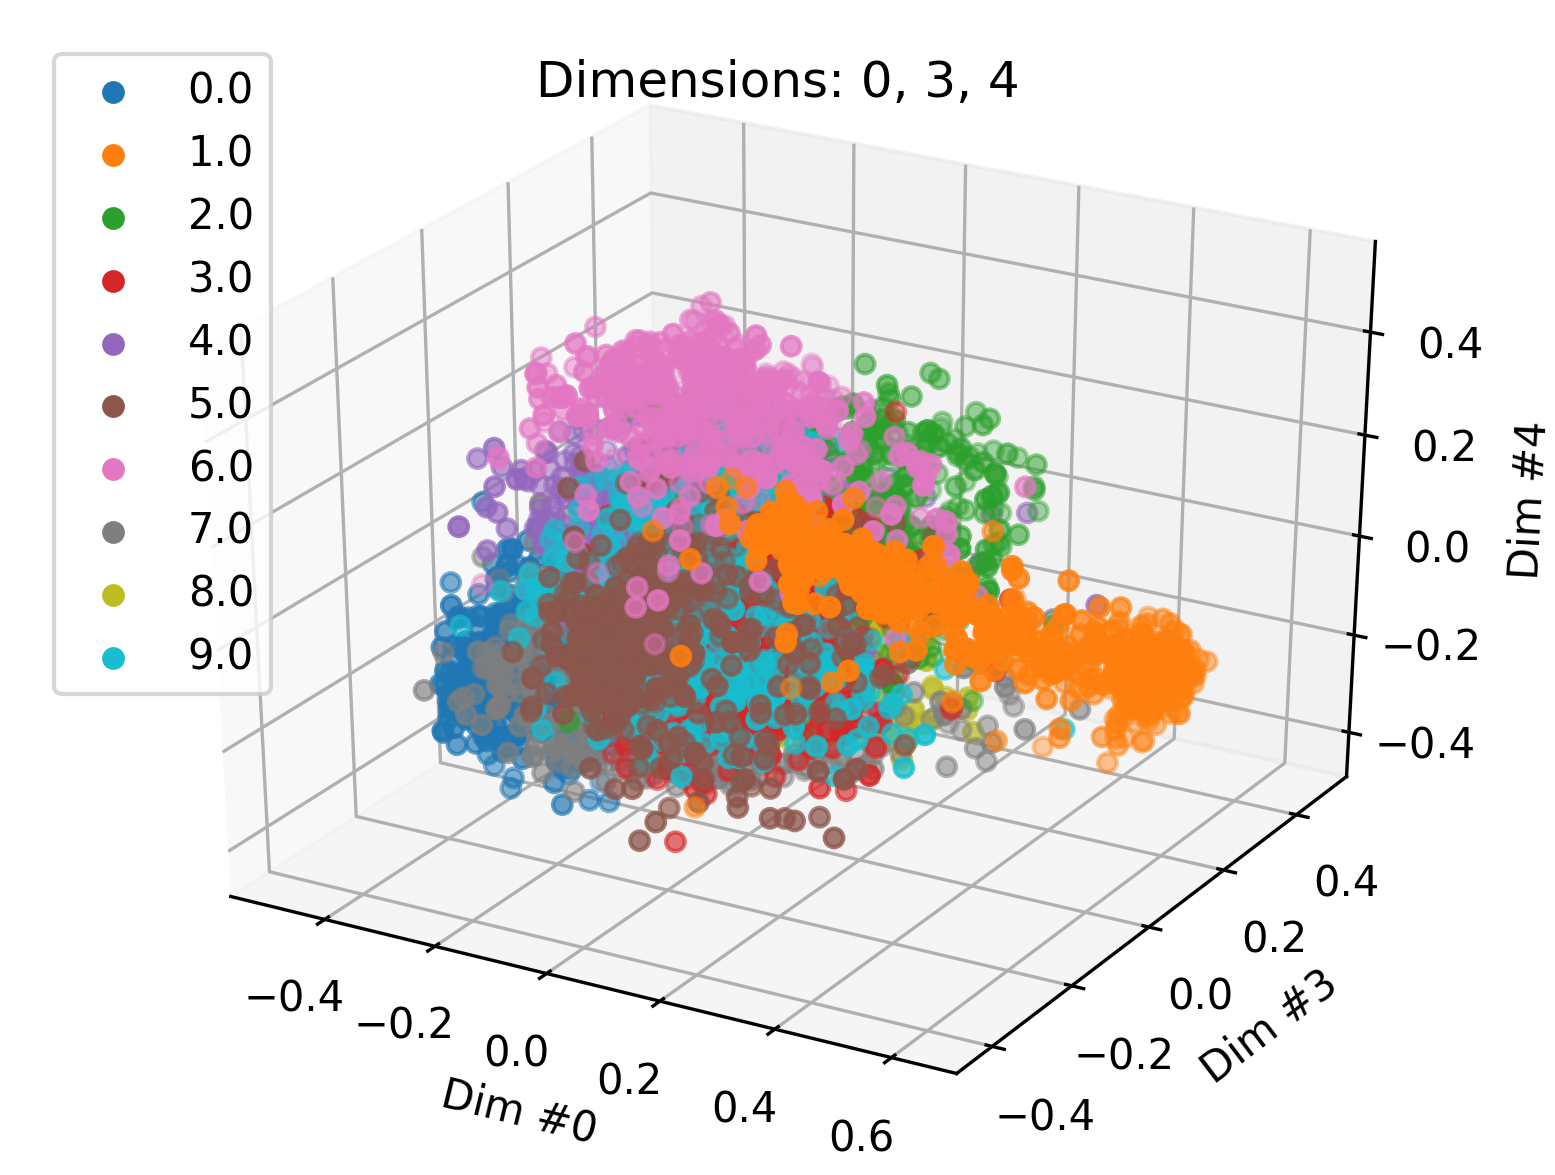
\includegraphics[width=0.23\textwidth]{pca/034.png}
  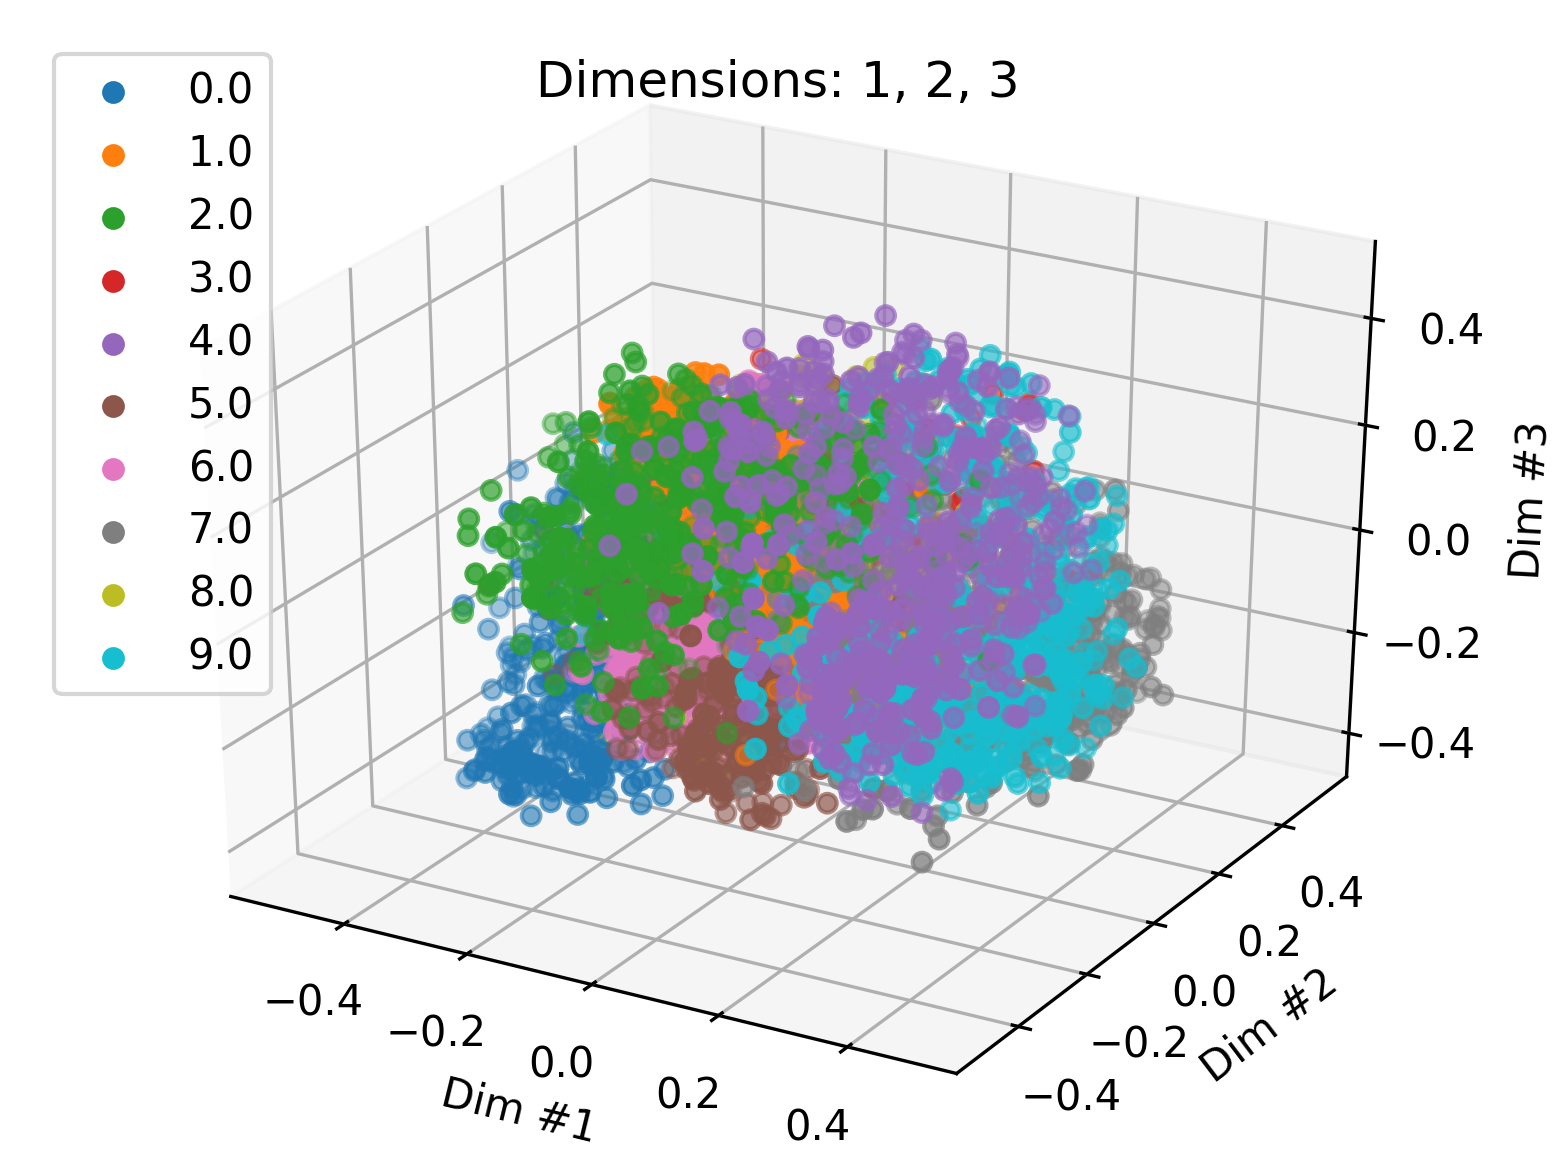
\includegraphics[width=0.23\textwidth]{pca/123.png}
  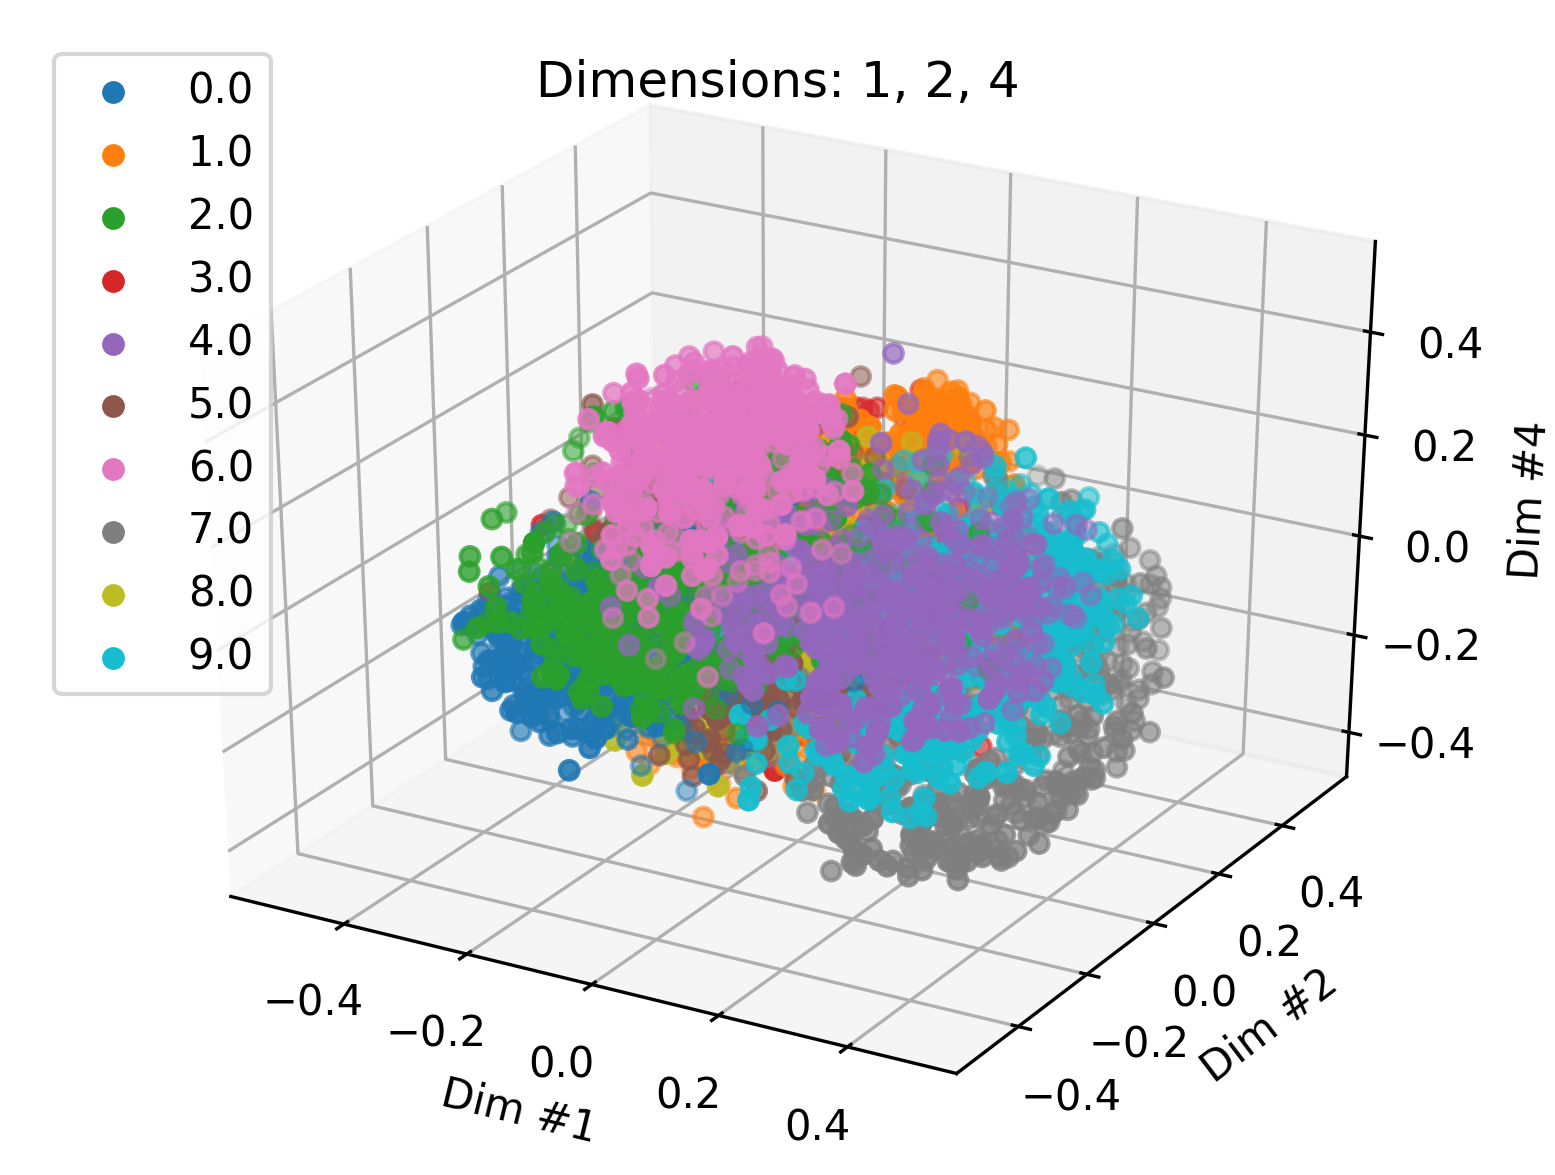
\includegraphics[width=0.23\textwidth]{pca/124.png}
  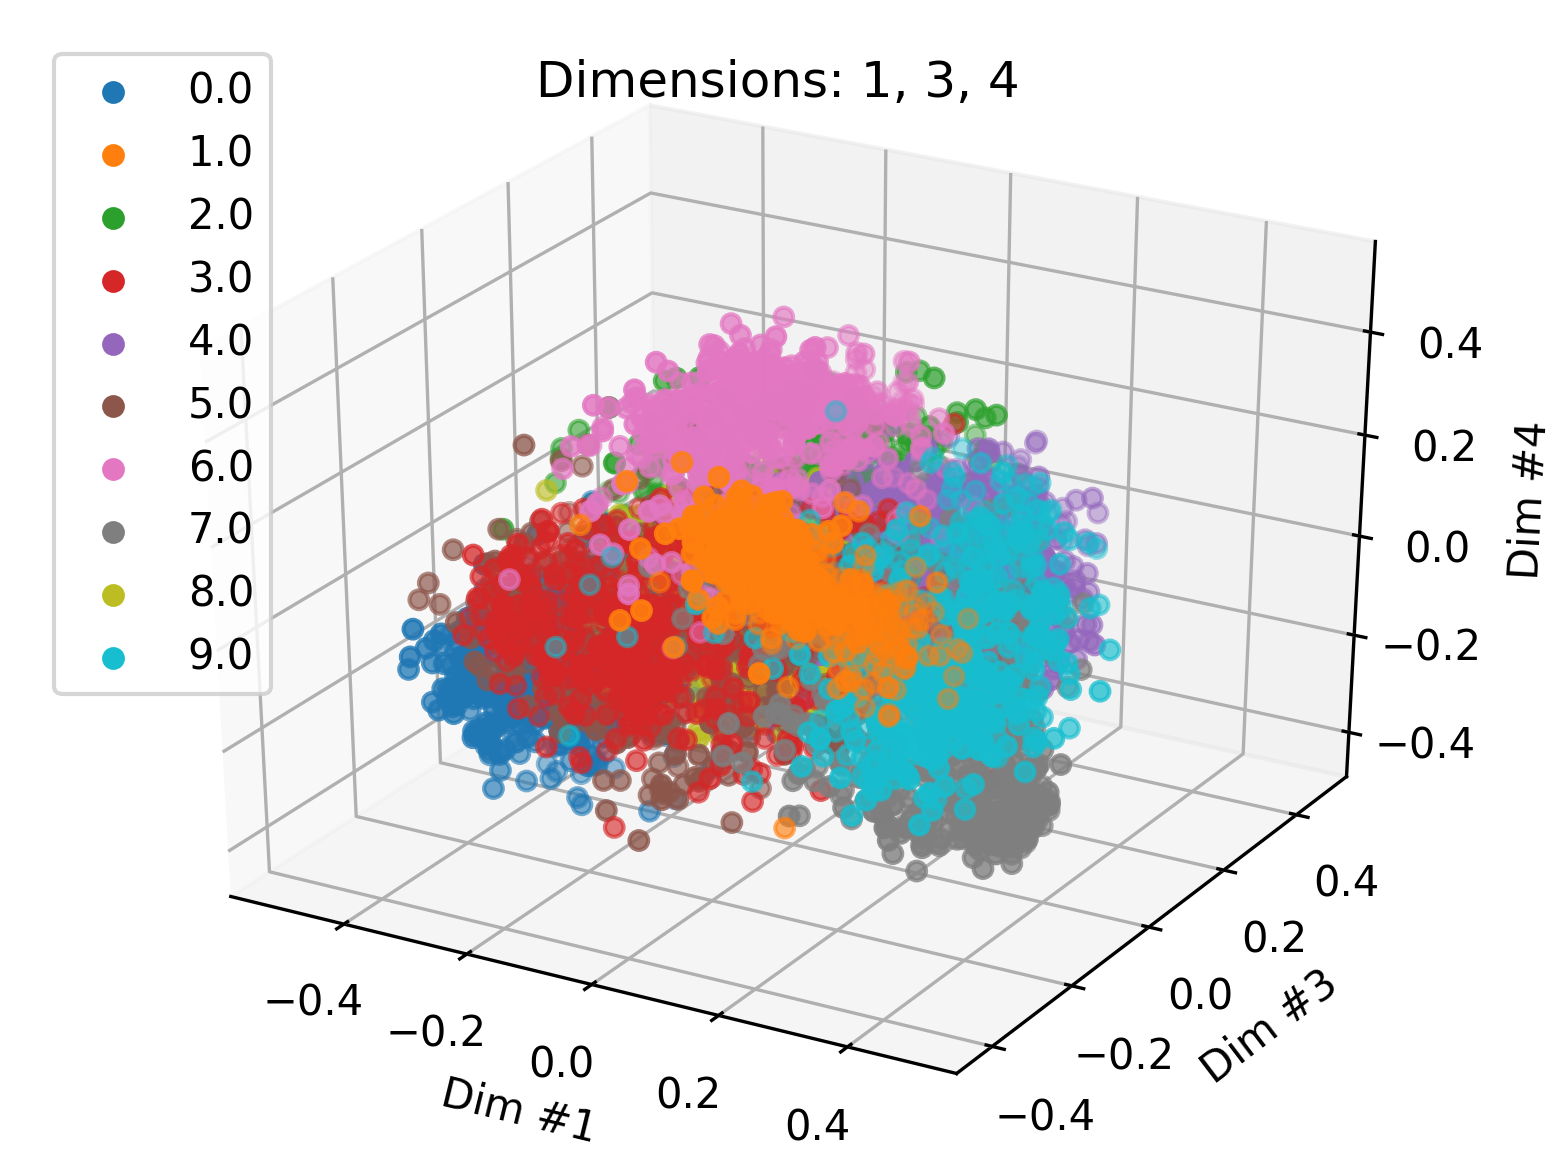
\includegraphics[width=0.23\textwidth]{pca/134.png}
  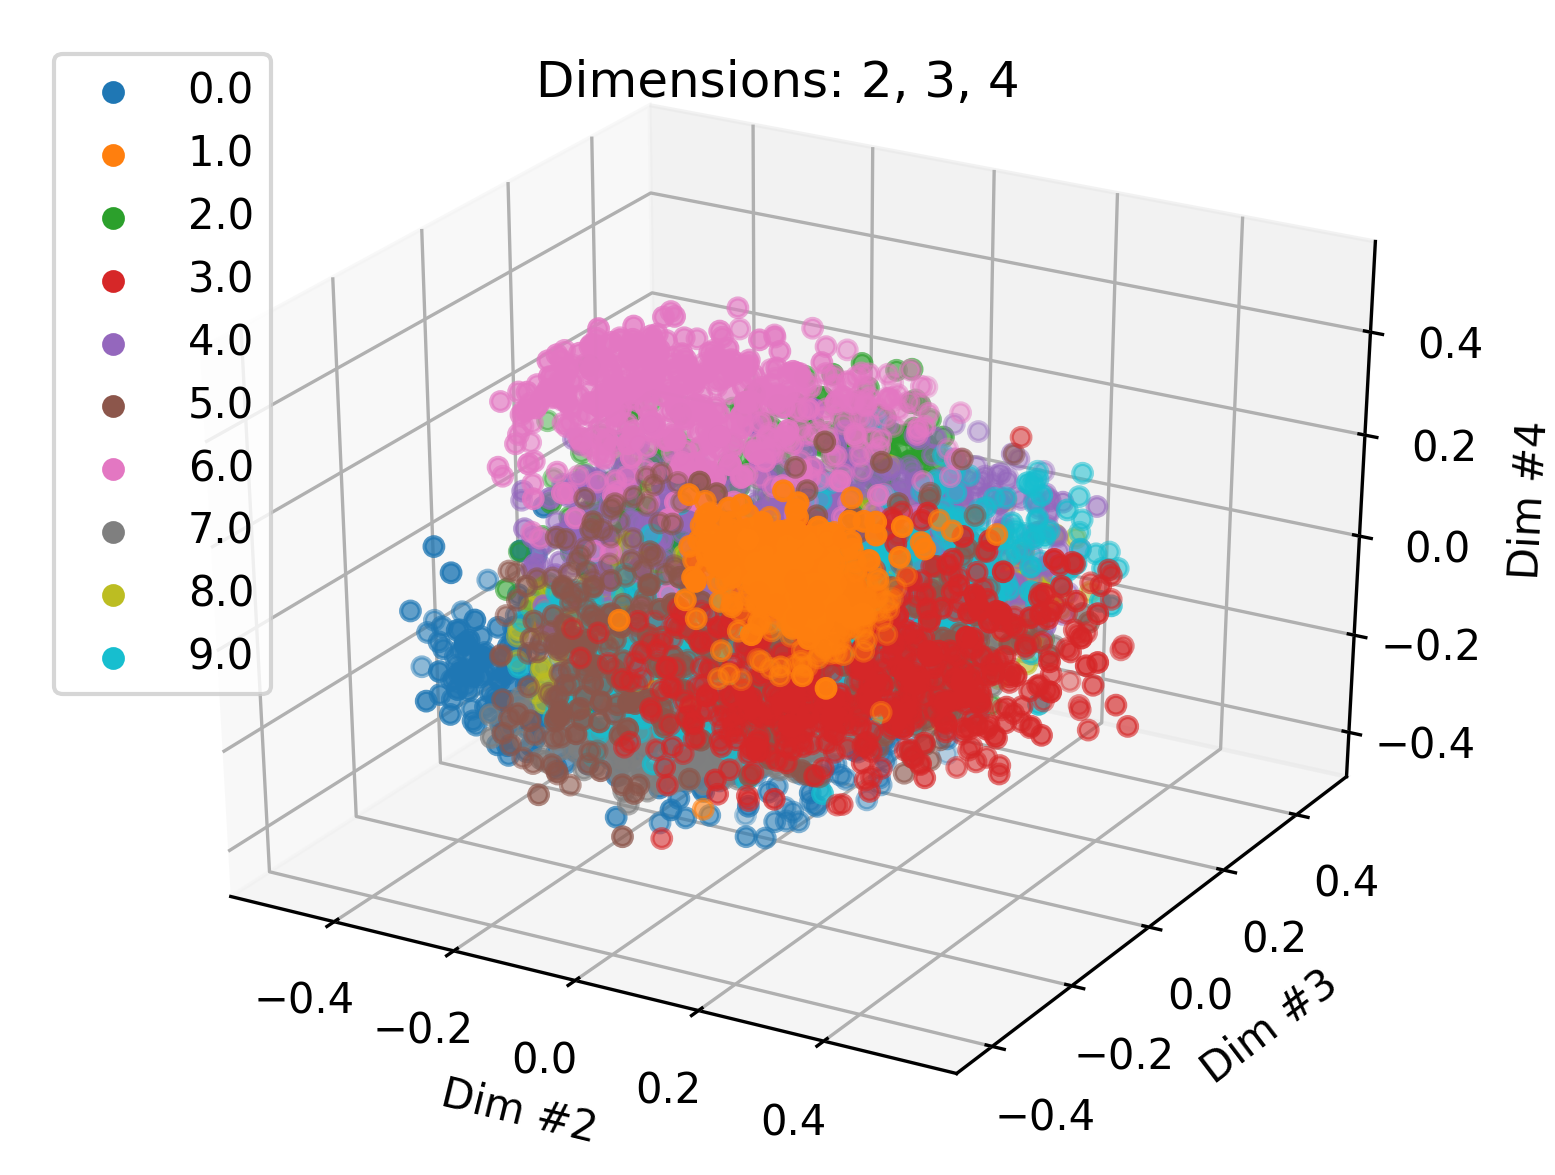
\includegraphics[width=0.23\textwidth]{pca/234.png}
  \caption{PCA graphs, coloured by the labels of the data. (Questions 2-6, part 1.)}
  \label{fig:pca_graphs}
\end{figure}

The `0'-labelled data points form distinct clusters in the figures containing
the zeroth dimension (i.e. the first principal component), but aside from this
it is difficult to identify distinct clusters in the data by eye.

To identify the most significant graph, we will use an informally-defined
measure of class separability --- i.e. in which graph the classes are the least
"mixed-up".  By eye, this seems to be either the graph with dimensions (0, 1,
3), as it has a very clearly distinct cluster for the `0'-labelled elements, or
the graph with dimensions (1, 2, 4), as it has fairly distinct class clusters.

For deeper analysis, an objective class separability measure could be used on
these 3-combinations of the principal components, but we will not do so
here.\footnote{This answers question 7 of part 1.}

\section{Competitive Learning} The model used for performing classification on
the dataset was a single-layer artificial neural network using a competitive
learning mode, as outlined in (REFERENCE).  Briefly, for an $n$-dimensional
input vector and $m$ output units, we randomly initialise $m{\times}n$ matrix
$W$ of initial artificial synapse weights.  Then, taking each input vector
$\bm{\xi}^\mu$ in turn, we compute $W\bm{\xi}^\mu$ to obtain an $m$-dimensional
vector of postsynaptic inputs.  To this, some noise is added and the
postsynaptic neuron with the hightest input firing rate is chosen to fire; all
other postsynaptic neurons do not fire.

For the learning step, the weights of the synapses connected to the winning
postsynaptic neuron are adjusted in proportion to the difference between their
previous weight and the input vector.  The constant of this proportion, $\eta$,
is termed the \textit{learning rate}, and is one of the parameters used in
tuning.  In fact, as per the recommendation in (REFERENCE), we decided to use a
decaying learning rate of $\eta(t) = \eta_0t^{-\alpha}$ for some $0 \le \alpha
\le 1$, where $\alpha$ is known as the rate of decay of the learning rate.

Since this method does not require us to present all the training vectors before
calculating the weights, we can conclude that it is an \textbf{online} learning
algorithm --- that is to say, the algorithm could be paused after any step and
used for evaluation, and indeed more training data can be presented at any
stage.

For the purposes of tuning, we use four parameters: the number of output units,
the learning rate, the weight of the added noise, and the rate of decay of the
learning rate.\footnote{This answers question 1 of part 2.  For further detail
and code snippets please see \autoref{sec:algorithms}.}

\section{Detailed Algorithms}
\label{sec:algorithms}
Something something

\end{document}
% Disable intented paragraphs and add space between them instead.
% \setlength{\parskip}{10pt}
% \setlength{\parindent}{0pt
